% Created by tikzDevice version 0.7.0 on 2014-07-29 02:50:08
% !TEX encoding = UTF-8 Unicode
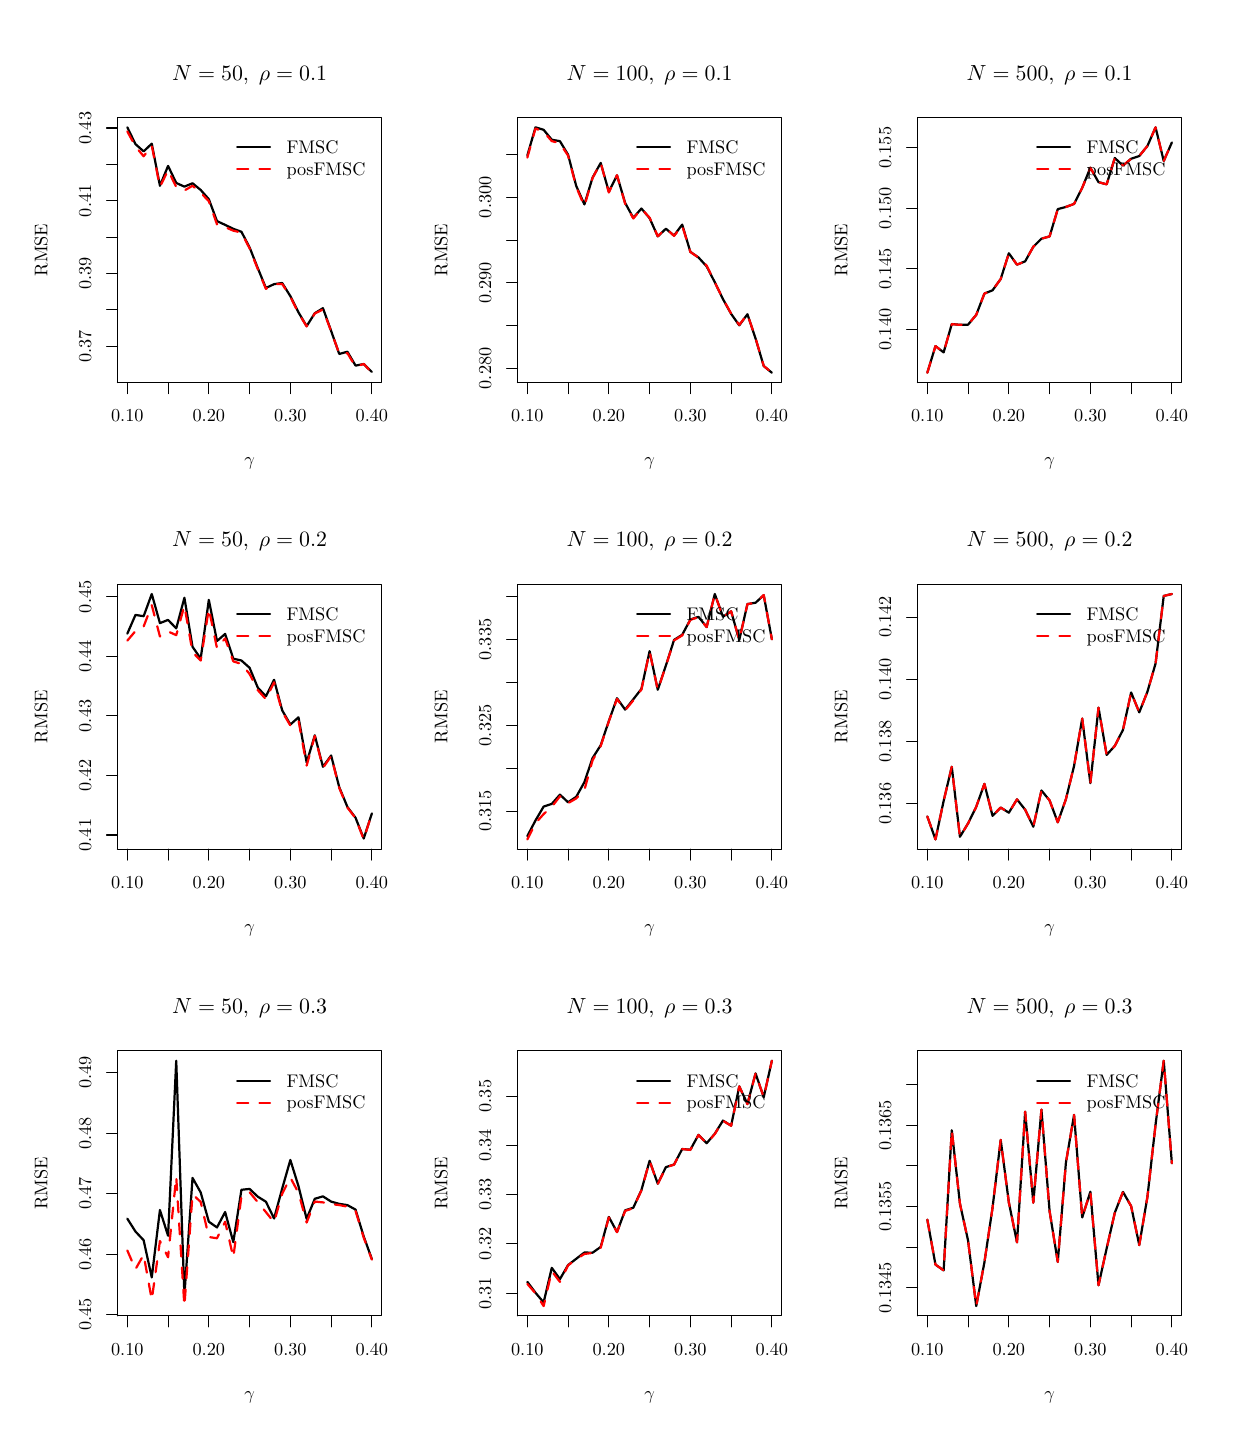
\begin{tikzpicture}[x=1pt,y=1pt]
\definecolor[named]{fillColor}{rgb}{1.00,1.00,1.00}
\path[use as bounding box,fill=fillColor,fill opacity=0.00] (0,0) rectangle (433.62,505.89);
\begin{scope}
\path[clip] ( 32.47,377.65) rectangle (127.91,473.42);
\definecolor[named]{drawColor}{rgb}{0.00,0.00,0.00}

\path[draw=drawColor,line width= 0.8pt,line join=round,line cap=round] ( 36.01,469.87) --
	( 38.95,463.81) --
	( 41.90,461.18) --
	( 44.84,463.97) --
	( 47.79,448.76) --
	( 50.73,455.93) --
	( 53.68,449.77) --
	( 56.63,448.45) --
	( 59.57,449.66) --
	( 62.52,447.24) --
	( 65.46,443.91) --
	( 68.41,435.98) --
	( 71.35,434.63) --
	( 74.30,433.20) --
	( 77.24,432.13) --
	( 80.19,426.48) --
	( 83.14,419.03) --
	( 86.08,411.83) --
	( 89.03,413.20) --
	( 91.97,413.62) --
	( 94.92,408.87) --
	( 97.86,403.01) --
	(100.81,398.03) --
	(103.75,402.71) --
	(106.70,404.52) --
	(109.65,396.31) --
	(112.59,387.98) --
	(115.54,388.79) --
	(118.48,383.77) --
	(121.43,384.34) --
	(124.37,381.48);
\end{scope}
\begin{scope}
\path[clip] (  0.00,  0.00) rectangle (433.62,505.89);
\definecolor[named]{drawColor}{rgb}{0.00,0.00,0.00}

\path[draw=drawColor,line width= 0.4pt,line join=round,line cap=round] ( 36.01,377.65) -- (124.37,377.65);

\path[draw=drawColor,line width= 0.4pt,line join=round,line cap=round] ( 36.01,377.65) -- ( 36.01,373.69);

\path[draw=drawColor,line width= 0.4pt,line join=round,line cap=round] ( 50.73,377.65) -- ( 50.73,373.69);

\path[draw=drawColor,line width= 0.4pt,line join=round,line cap=round] ( 65.46,377.65) -- ( 65.46,373.69);

\path[draw=drawColor,line width= 0.4pt,line join=round,line cap=round] ( 80.19,377.65) -- ( 80.19,373.69);

\path[draw=drawColor,line width= 0.4pt,line join=round,line cap=round] ( 94.92,377.65) -- ( 94.92,373.69);

\path[draw=drawColor,line width= 0.4pt,line join=round,line cap=round] (109.65,377.65) -- (109.65,373.69);

\path[draw=drawColor,line width= 0.4pt,line join=round,line cap=round] (124.37,377.65) -- (124.37,373.69);

\node[text=drawColor,anchor=base,inner sep=0pt, outer sep=0pt, scale=  0.66] at ( 36.01,363.40) {0.10};

\node[text=drawColor,anchor=base,inner sep=0pt, outer sep=0pt, scale=  0.66] at ( 65.46,363.40) {0.20};

\node[text=drawColor,anchor=base,inner sep=0pt, outer sep=0pt, scale=  0.66] at ( 94.92,363.40) {0.30};

\node[text=drawColor,anchor=base,inner sep=0pt, outer sep=0pt, scale=  0.66] at (124.37,363.40) {0.40};

\path[draw=drawColor,line width= 0.4pt,line join=round,line cap=round] ( 32.47,390.75) -- ( 32.47,469.63);

\path[draw=drawColor,line width= 0.4pt,line join=round,line cap=round] ( 32.47,390.75) -- ( 28.51,390.75);

\path[draw=drawColor,line width= 0.4pt,line join=round,line cap=round] ( 32.47,403.89) -- ( 28.51,403.89);

\path[draw=drawColor,line width= 0.4pt,line join=round,line cap=round] ( 32.47,417.04) -- ( 28.51,417.04);

\path[draw=drawColor,line width= 0.4pt,line join=round,line cap=round] ( 32.47,430.19) -- ( 28.51,430.19);

\path[draw=drawColor,line width= 0.4pt,line join=round,line cap=round] ( 32.47,443.33) -- ( 28.51,443.33);

\path[draw=drawColor,line width= 0.4pt,line join=round,line cap=round] ( 32.47,456.48) -- ( 28.51,456.48);

\path[draw=drawColor,line width= 0.4pt,line join=round,line cap=round] ( 32.47,469.63) -- ( 28.51,469.63);

\node[text=drawColor,rotate= 90.00,anchor=base,inner sep=0pt, outer sep=0pt, scale=  0.66] at ( 22.97,390.75) {0.37};

\node[text=drawColor,rotate= 90.00,anchor=base,inner sep=0pt, outer sep=0pt, scale=  0.66] at ( 22.97,417.04) {0.39};

\node[text=drawColor,rotate= 90.00,anchor=base,inner sep=0pt, outer sep=0pt, scale=  0.66] at ( 22.97,443.33) {0.41};

\node[text=drawColor,rotate= 90.00,anchor=base,inner sep=0pt, outer sep=0pt, scale=  0.66] at ( 22.97,469.63) {0.43};

\path[draw=drawColor,line width= 0.4pt,line join=round,line cap=round] ( 32.47,377.65) --
	(127.91,377.65) --
	(127.91,473.42) --
	( 32.47,473.42) --
	( 32.47,377.65);
\end{scope}
\begin{scope}
\path[clip] (  0.00,337.26) rectangle (144.54,505.89);
\definecolor[named]{drawColor}{rgb}{0.00,0.00,0.00}

\node[text=drawColor,anchor=base,inner sep=0pt, outer sep=0pt, scale=  0.79] at ( 80.19,486.92) {\bfseries $N=50, \;\rho=0.1$};

\node[text=drawColor,anchor=base,inner sep=0pt, outer sep=0pt, scale=  0.66] at ( 80.19,347.56) {$\gamma$};

\node[text=drawColor,rotate= 90.00,anchor=base,inner sep=0pt, outer sep=0pt, scale=  0.66] at (  7.13,425.53) {RMSE};
\end{scope}
\begin{scope}
\path[clip] ( 32.47,377.65) rectangle (127.91,473.42);
\definecolor[named]{drawColor}{rgb}{1.00,0.00,0.00}

\path[draw=drawColor,line width= 0.8pt,dash pattern=on 4pt off 4pt ,line join=round,line cap=round] ( 36.01,468.39) --
	( 38.95,462.97) --
	( 41.90,459.41) --
	( 44.84,463.27) --
	( 47.79,448.34) --
	( 50.73,454.39) --
	( 53.68,448.31) --
	( 56.63,447.04) --
	( 59.57,448.76) --
	( 62.52,446.24) --
	( 65.46,443.19) --
	( 68.41,434.82) --
	( 71.35,433.81) --
	( 74.30,432.54) --
	( 77.24,431.84) --
	( 80.19,426.14) --
	( 83.14,418.67) --
	( 86.08,411.51) --
	( 89.03,413.21) --
	( 91.97,413.28) --
	( 94.92,408.68) --
	( 97.86,402.68) --
	(100.81,397.94) --
	(103.75,402.62) --
	(106.70,404.04) --
	(109.65,396.20) --
	(112.59,388.05) --
	(115.54,388.29) --
	(118.48,383.35) --
	(121.43,384.37) --
	(124.37,381.20);
\definecolor[named]{drawColor}{rgb}{0.00,0.00,0.00}

\path[draw=drawColor,line width= 0.8pt,line join=round,line cap=round] ( 75.72,462.63) -- ( 87.60,462.63);
\definecolor[named]{drawColor}{rgb}{1.00,0.00,0.00}

\path[draw=drawColor,line width= 0.8pt,dash pattern=on 4pt off 4pt ,line join=round,line cap=round] ( 75.72,454.71) -- ( 87.60,454.71);
\definecolor[named]{drawColor}{rgb}{0.00,0.00,0.00}

\node[text=drawColor,anchor=base west,inner sep=0pt, outer sep=0pt, scale=  0.66] at ( 93.54,460.35) {FMSC};

\node[text=drawColor,anchor=base west,inner sep=0pt, outer sep=0pt, scale=  0.66] at ( 93.54,452.43) {posFMSC};
\end{scope}
\begin{scope}
\path[clip] (177.01,377.65) rectangle (272.45,473.42);
\definecolor[named]{drawColor}{rgb}{0.00,0.00,0.00}

\path[draw=drawColor,line width= 0.8pt,line join=round,line cap=round] (180.55,459.68) --
	(183.49,469.87) --
	(186.44,468.98) --
	(189.38,465.40) --
	(192.33,464.87) --
	(195.27,459.99) --
	(198.22,448.68) --
	(201.17,442.02) --
	(204.11,451.67) --
	(207.06,457.01) --
	(210.00,446.61) --
	(212.95,452.51) --
	(215.89,442.58) --
	(218.84,437.17) --
	(221.78,440.53) --
	(224.73,437.06) --
	(227.68,430.46) --
	(230.62,433.23) --
	(233.57,430.77) --
	(236.51,434.73) --
	(239.46,424.87) --
	(242.40,422.85) --
	(245.35,419.62) --
	(248.29,413.89) --
	(251.24,407.81) --
	(254.19,402.47) --
	(257.13,398.32) --
	(260.08,402.33) --
	(263.02,393.58) --
	(265.97,383.62) --
	(268.91,381.20);
\end{scope}
\begin{scope}
\path[clip] (  0.00,  0.00) rectangle (433.62,505.89);
\definecolor[named]{drawColor}{rgb}{0.00,0.00,0.00}

\path[draw=drawColor,line width= 0.4pt,line join=round,line cap=round] (180.55,377.65) -- (268.91,377.65);

\path[draw=drawColor,line width= 0.4pt,line join=round,line cap=round] (180.55,377.65) -- (180.55,373.69);

\path[draw=drawColor,line width= 0.4pt,line join=round,line cap=round] (195.27,377.65) -- (195.27,373.69);

\path[draw=drawColor,line width= 0.4pt,line join=round,line cap=round] (210.00,377.65) -- (210.00,373.69);

\path[draw=drawColor,line width= 0.4pt,line join=round,line cap=round] (224.73,377.65) -- (224.73,373.69);

\path[draw=drawColor,line width= 0.4pt,line join=round,line cap=round] (239.46,377.65) -- (239.46,373.69);

\path[draw=drawColor,line width= 0.4pt,line join=round,line cap=round] (254.19,377.65) -- (254.19,373.69);

\path[draw=drawColor,line width= 0.4pt,line join=round,line cap=round] (268.91,377.65) -- (268.91,373.69);

\node[text=drawColor,anchor=base,inner sep=0pt, outer sep=0pt, scale=  0.66] at (180.55,363.40) {0.10};

\node[text=drawColor,anchor=base,inner sep=0pt, outer sep=0pt, scale=  0.66] at (210.00,363.40) {0.20};

\node[text=drawColor,anchor=base,inner sep=0pt, outer sep=0pt, scale=  0.66] at (239.46,363.40) {0.30};

\node[text=drawColor,anchor=base,inner sep=0pt, outer sep=0pt, scale=  0.66] at (268.91,363.40) {0.40};

\path[draw=drawColor,line width= 0.4pt,line join=round,line cap=round] (177.01,382.79) -- (177.01,460.04);

\path[draw=drawColor,line width= 0.4pt,line join=round,line cap=round] (177.01,382.79) -- (173.05,382.79);

\path[draw=drawColor,line width= 0.4pt,line join=round,line cap=round] (177.01,398.24) -- (173.05,398.24);

\path[draw=drawColor,line width= 0.4pt,line join=round,line cap=round] (177.01,413.69) -- (173.05,413.69);

\path[draw=drawColor,line width= 0.4pt,line join=round,line cap=round] (177.01,429.14) -- (173.05,429.14);

\path[draw=drawColor,line width= 0.4pt,line join=round,line cap=round] (177.01,444.59) -- (173.05,444.59);

\path[draw=drawColor,line width= 0.4pt,line join=round,line cap=round] (177.01,460.04) -- (173.05,460.04);

\node[text=drawColor,rotate= 90.00,anchor=base,inner sep=0pt, outer sep=0pt, scale=  0.66] at (167.51,382.79) {0.280};

\node[text=drawColor,rotate= 90.00,anchor=base,inner sep=0pt, outer sep=0pt, scale=  0.66] at (167.51,413.69) {0.290};

\node[text=drawColor,rotate= 90.00,anchor=base,inner sep=0pt, outer sep=0pt, scale=  0.66] at (167.51,444.59) {0.300};

\path[draw=drawColor,line width= 0.4pt,line join=round,line cap=round] (177.01,377.65) --
	(272.45,377.65) --
	(272.45,473.42) --
	(177.01,473.42) --
	(177.01,377.65);
\end{scope}
\begin{scope}
\path[clip] (144.54,337.26) rectangle (289.08,505.89);
\definecolor[named]{drawColor}{rgb}{0.00,0.00,0.00}

\node[text=drawColor,anchor=base,inner sep=0pt, outer sep=0pt, scale=  0.79] at (224.73,486.92) {\bfseries $N=100, \;\rho=0.1$};

\node[text=drawColor,anchor=base,inner sep=0pt, outer sep=0pt, scale=  0.66] at (224.73,347.56) {$\gamma$};

\node[text=drawColor,rotate= 90.00,anchor=base,inner sep=0pt, outer sep=0pt, scale=  0.66] at (151.67,425.54) {RMSE};
\end{scope}
\begin{scope}
\path[clip] (177.01,377.65) rectangle (272.45,473.42);
\definecolor[named]{drawColor}{rgb}{1.00,0.00,0.00}

\path[draw=drawColor,line width= 0.8pt,dash pattern=on 4pt off 4pt ,line join=round,line cap=round] (180.55,458.94) --
	(183.49,469.44) --
	(186.44,468.26) --
	(189.38,464.90) --
	(192.33,464.13) --
	(195.27,459.67) --
	(198.22,448.36) --
	(201.17,441.39) --
	(204.11,451.56) --
	(207.06,457.03) --
	(210.00,446.32) --
	(212.95,452.60) --
	(215.89,442.26) --
	(218.84,436.93) --
	(221.78,440.44) --
	(224.73,437.21) --
	(227.68,430.52) --
	(230.62,433.36) --
	(233.57,430.64) --
	(236.51,434.37) --
	(239.46,424.84) --
	(242.40,422.81) --
	(245.35,419.91) --
	(248.29,413.84) --
	(251.24,407.84) --
	(254.19,402.56) --
	(257.13,398.49) --
	(260.08,402.35) --
	(263.02,393.67) --
	(265.97,383.65) --
	(268.91,381.24);
\definecolor[named]{drawColor}{rgb}{0.00,0.00,0.00}

\path[draw=drawColor,line width= 0.8pt,line join=round,line cap=round] (220.26,462.63) -- (232.14,462.63);
\definecolor[named]{drawColor}{rgb}{1.00,0.00,0.00}

\path[draw=drawColor,line width= 0.8pt,dash pattern=on 4pt off 4pt ,line join=round,line cap=round] (220.26,454.71) -- (232.14,454.71);
\definecolor[named]{drawColor}{rgb}{0.00,0.00,0.00}

\node[text=drawColor,anchor=base west,inner sep=0pt, outer sep=0pt, scale=  0.66] at (238.08,460.35) {FMSC};

\node[text=drawColor,anchor=base west,inner sep=0pt, outer sep=0pt, scale=  0.66] at (238.08,452.43) {posFMSC};
\end{scope}
\begin{scope}
\path[clip] (321.55,377.65) rectangle (416.99,473.42);
\definecolor[named]{drawColor}{rgb}{0.00,0.00,0.00}

\path[draw=drawColor,line width= 0.8pt,line join=round,line cap=round] (325.09,381.23) --
	(328.03,390.83) --
	(330.98,388.55) --
	(333.92,398.79) --
	(336.87,398.52) --
	(339.81,398.57) --
	(342.76,402.12) --
	(345.71,409.81) --
	(348.65,410.98) --
	(351.60,415.06) --
	(354.54,424.36) --
	(357.49,420.25) --
	(360.43,421.44) --
	(363.38,426.72) --
	(366.32,429.63) --
	(369.27,430.46) --
	(372.22,440.32) --
	(375.16,441.10) --
	(378.11,442.20) --
	(381.05,448.00) --
	(384.00,455.29) --
	(386.94,450.06) --
	(389.89,449.27) --
	(392.83,458.78) --
	(395.78,456.05) --
	(398.73,458.51) --
	(401.67,459.51) --
	(404.62,463.14) --
	(407.56,469.87) --
	(410.51,457.71) --
	(413.45,464.41);
\end{scope}
\begin{scope}
\path[clip] (  0.00,  0.00) rectangle (433.62,505.89);
\definecolor[named]{drawColor}{rgb}{0.00,0.00,0.00}

\path[draw=drawColor,line width= 0.4pt,line join=round,line cap=round] (325.09,377.65) -- (413.45,377.65);

\path[draw=drawColor,line width= 0.4pt,line join=round,line cap=round] (325.09,377.65) -- (325.09,373.69);

\path[draw=drawColor,line width= 0.4pt,line join=round,line cap=round] (339.81,377.65) -- (339.81,373.69);

\path[draw=drawColor,line width= 0.4pt,line join=round,line cap=round] (354.54,377.65) -- (354.54,373.69);

\path[draw=drawColor,line width= 0.4pt,line join=round,line cap=round] (369.27,377.65) -- (369.27,373.69);

\path[draw=drawColor,line width= 0.4pt,line join=round,line cap=round] (384.00,377.65) -- (384.00,373.69);

\path[draw=drawColor,line width= 0.4pt,line join=round,line cap=round] (398.73,377.65) -- (398.73,373.69);

\path[draw=drawColor,line width= 0.4pt,line join=round,line cap=round] (413.45,377.65) -- (413.45,373.69);

\node[text=drawColor,anchor=base,inner sep=0pt, outer sep=0pt, scale=  0.66] at (325.09,363.40) {0.10};

\node[text=drawColor,anchor=base,inner sep=0pt, outer sep=0pt, scale=  0.66] at (354.54,363.40) {0.20};

\node[text=drawColor,anchor=base,inner sep=0pt, outer sep=0pt, scale=  0.66] at (384.00,363.40) {0.30};

\node[text=drawColor,anchor=base,inner sep=0pt, outer sep=0pt, scale=  0.66] at (413.45,363.40) {0.40};

\path[draw=drawColor,line width= 0.4pt,line join=round,line cap=round] (321.55,396.83) -- (321.55,462.55);

\path[draw=drawColor,line width= 0.4pt,line join=round,line cap=round] (321.55,396.83) -- (317.59,396.83);

\path[draw=drawColor,line width= 0.4pt,line join=round,line cap=round] (321.55,418.73) -- (317.59,418.73);

\path[draw=drawColor,line width= 0.4pt,line join=round,line cap=round] (321.55,440.64) -- (317.59,440.64);

\path[draw=drawColor,line width= 0.4pt,line join=round,line cap=round] (321.55,462.55) -- (317.59,462.55);

\node[text=drawColor,rotate= 90.00,anchor=base,inner sep=0pt, outer sep=0pt, scale=  0.66] at (312.05,396.83) {0.140};

\node[text=drawColor,rotate= 90.00,anchor=base,inner sep=0pt, outer sep=0pt, scale=  0.66] at (312.05,418.73) {0.145};

\node[text=drawColor,rotate= 90.00,anchor=base,inner sep=0pt, outer sep=0pt, scale=  0.66] at (312.05,440.64) {0.150};

\node[text=drawColor,rotate= 90.00,anchor=base,inner sep=0pt, outer sep=0pt, scale=  0.66] at (312.05,462.55) {0.155};

\path[draw=drawColor,line width= 0.4pt,line join=round,line cap=round] (321.55,377.65) --
	(416.99,377.65) --
	(416.99,473.42) --
	(321.55,473.42) --
	(321.55,377.65);
\end{scope}
\begin{scope}
\path[clip] (289.08,337.26) rectangle (433.62,505.89);
\definecolor[named]{drawColor}{rgb}{0.00,0.00,0.00}

\node[text=drawColor,anchor=base,inner sep=0pt, outer sep=0pt, scale=  0.79] at (369.27,486.92) {\bfseries $N=500, \;\rho=0.1$};

\node[text=drawColor,anchor=base,inner sep=0pt, outer sep=0pt, scale=  0.66] at (369.27,347.56) {$\gamma$};

\node[text=drawColor,rotate= 90.00,anchor=base,inner sep=0pt, outer sep=0pt, scale=  0.66] at (296.21,425.53) {RMSE};
\end{scope}
\begin{scope}
\path[clip] (321.55,377.65) rectangle (416.99,473.42);
\definecolor[named]{drawColor}{rgb}{1.00,0.00,0.00}

\path[draw=drawColor,line width= 0.8pt,dash pattern=on 4pt off 4pt ,line join=round,line cap=round] (325.09,381.20) --
	(328.03,390.82) --
	(330.98,388.54) --
	(333.92,398.75) --
	(336.87,398.50) --
	(339.81,398.58) --
	(342.76,402.12) --
	(345.71,409.81) --
	(348.65,410.99) --
	(351.60,415.07) --
	(354.54,424.36) --
	(357.49,420.25) --
	(360.43,421.44) --
	(363.38,426.72) --
	(366.32,429.63) --
	(369.27,430.46) --
	(372.22,440.32) --
	(375.16,441.10) --
	(378.11,442.20) --
	(381.05,448.00) --
	(384.00,455.29) --
	(386.94,450.06) --
	(389.89,449.27) --
	(392.83,458.78) --
	(395.78,456.05) --
	(398.73,458.51) --
	(401.67,459.51) --
	(404.62,463.14) --
	(407.56,469.87) --
	(410.51,457.71) --
	(413.45,464.41);
\definecolor[named]{drawColor}{rgb}{0.00,0.00,0.00}

\path[draw=drawColor,line width= 0.8pt,line join=round,line cap=round] (364.80,462.63) -- (376.68,462.63);
\definecolor[named]{drawColor}{rgb}{1.00,0.00,0.00}

\path[draw=drawColor,line width= 0.8pt,dash pattern=on 4pt off 4pt ,line join=round,line cap=round] (364.80,454.71) -- (376.68,454.71);
\definecolor[named]{drawColor}{rgb}{0.00,0.00,0.00}

\node[text=drawColor,anchor=base west,inner sep=0pt, outer sep=0pt, scale=  0.66] at (382.62,460.35) {FMSC};

\node[text=drawColor,anchor=base west,inner sep=0pt, outer sep=0pt, scale=  0.66] at (382.62,452.43) {posFMSC};
\end{scope}
\begin{scope}
\path[clip] ( 32.47,209.02) rectangle (127.91,304.79);
\definecolor[named]{drawColor}{rgb}{0.00,0.00,0.00}

\path[draw=drawColor,line width= 0.8pt,line join=round,line cap=round] ( 36.01,286.92) --
	( 38.95,293.68) --
	( 41.90,293.22) --
	( 44.84,301.24) --
	( 47.79,290.72) --
	( 50.73,291.88) --
	( 53.68,288.81) --
	( 56.63,299.88) --
	( 59.57,282.17) --
	( 62.52,277.90) --
	( 65.46,299.13) --
	( 68.41,284.24) --
	( 71.35,286.83) --
	( 74.30,277.87) --
	( 77.24,277.21) --
	( 80.19,274.58) --
	( 83.14,267.44) --
	( 86.08,264.28) --
	( 89.03,270.23) --
	( 91.97,259.20) --
	( 94.92,254.07) --
	( 97.86,256.69) --
	(100.81,240.36) --
	(103.75,250.18) --
	(106.70,238.80) --
	(109.65,242.89) --
	(112.59,231.43) --
	(115.54,224.30) --
	(118.48,220.38) --
	(121.43,212.89) --
	(124.37,221.95);
\end{scope}
\begin{scope}
\path[clip] (  0.00,  0.00) rectangle (433.62,505.89);
\definecolor[named]{drawColor}{rgb}{0.00,0.00,0.00}

\path[draw=drawColor,line width= 0.4pt,line join=round,line cap=round] ( 36.01,209.02) -- (124.37,209.02);

\path[draw=drawColor,line width= 0.4pt,line join=round,line cap=round] ( 36.01,209.02) -- ( 36.01,205.06);

\path[draw=drawColor,line width= 0.4pt,line join=round,line cap=round] ( 50.73,209.02) -- ( 50.73,205.06);

\path[draw=drawColor,line width= 0.4pt,line join=round,line cap=round] ( 65.46,209.02) -- ( 65.46,205.06);

\path[draw=drawColor,line width= 0.4pt,line join=round,line cap=round] ( 80.19,209.02) -- ( 80.19,205.06);

\path[draw=drawColor,line width= 0.4pt,line join=round,line cap=round] ( 94.92,209.02) -- ( 94.92,205.06);

\path[draw=drawColor,line width= 0.4pt,line join=round,line cap=round] (109.65,209.02) -- (109.65,205.06);

\path[draw=drawColor,line width= 0.4pt,line join=round,line cap=round] (124.37,209.02) -- (124.37,205.06);

\node[text=drawColor,anchor=base,inner sep=0pt, outer sep=0pt, scale=  0.66] at ( 36.01,194.77) {0.10};

\node[text=drawColor,anchor=base,inner sep=0pt, outer sep=0pt, scale=  0.66] at ( 65.46,194.77) {0.20};

\node[text=drawColor,anchor=base,inner sep=0pt, outer sep=0pt, scale=  0.66] at ( 94.92,194.77) {0.30};

\node[text=drawColor,anchor=base,inner sep=0pt, outer sep=0pt, scale=  0.66] at (124.37,194.77) {0.40};

\path[draw=drawColor,line width= 0.4pt,line join=round,line cap=round] ( 32.47,214.16) -- ( 32.47,300.24);

\path[draw=drawColor,line width= 0.4pt,line join=round,line cap=round] ( 32.47,214.16) -- ( 28.51,214.16);

\path[draw=drawColor,line width= 0.4pt,line join=round,line cap=round] ( 32.47,235.68) -- ( 28.51,235.68);

\path[draw=drawColor,line width= 0.4pt,line join=round,line cap=round] ( 32.47,257.20) -- ( 28.51,257.20);

\path[draw=drawColor,line width= 0.4pt,line join=round,line cap=round] ( 32.47,278.72) -- ( 28.51,278.72);

\path[draw=drawColor,line width= 0.4pt,line join=round,line cap=round] ( 32.47,300.24) -- ( 28.51,300.24);

\node[text=drawColor,rotate= 90.00,anchor=base,inner sep=0pt, outer sep=0pt, scale=  0.66] at ( 22.97,214.16) {0.41};

\node[text=drawColor,rotate= 90.00,anchor=base,inner sep=0pt, outer sep=0pt, scale=  0.66] at ( 22.97,235.68) {0.42};

\node[text=drawColor,rotate= 90.00,anchor=base,inner sep=0pt, outer sep=0pt, scale=  0.66] at ( 22.97,257.20) {0.43};

\node[text=drawColor,rotate= 90.00,anchor=base,inner sep=0pt, outer sep=0pt, scale=  0.66] at ( 22.97,278.72) {0.44};

\node[text=drawColor,rotate= 90.00,anchor=base,inner sep=0pt, outer sep=0pt, scale=  0.66] at ( 22.97,300.24) {0.45};

\path[draw=drawColor,line width= 0.4pt,line join=round,line cap=round] ( 32.47,209.02) --
	(127.91,209.02) --
	(127.91,304.79) --
	( 32.47,304.79) --
	( 32.47,209.02);
\end{scope}
\begin{scope}
\path[clip] (  0.00,168.63) rectangle (144.54,337.26);
\definecolor[named]{drawColor}{rgb}{0.00,0.00,0.00}

\node[text=drawColor,anchor=base,inner sep=0pt, outer sep=0pt, scale=  0.79] at ( 80.19,318.29) {\bfseries $N=50, \;\rho=0.2$};

\node[text=drawColor,anchor=base,inner sep=0pt, outer sep=0pt, scale=  0.66] at ( 80.19,178.93) {$\gamma$};

\node[text=drawColor,rotate= 90.00,anchor=base,inner sep=0pt, outer sep=0pt, scale=  0.66] at (  7.13,256.91) {RMSE};
\end{scope}
\begin{scope}
\path[clip] ( 32.47,209.02) rectangle (127.91,304.79);
\definecolor[named]{drawColor}{rgb}{1.00,0.00,0.00}

\path[draw=drawColor,line width= 0.8pt,dash pattern=on 4pt off 4pt ,line join=round,line cap=round] ( 36.01,284.39) --
	( 38.95,287.86) --
	( 41.90,289.49) --
	( 44.84,297.18) --
	( 47.79,285.90) --
	( 50.73,287.72) --
	( 53.68,286.37) --
	( 56.63,297.01) --
	( 59.57,280.23) --
	( 62.52,277.19) --
	( 65.46,295.96) --
	( 68.41,281.64) --
	( 71.35,285.18) --
	( 74.30,276.90) --
	( 77.24,275.95) --
	( 80.19,272.34) --
	( 83.14,266.52) --
	( 86.08,263.23) --
	( 89.03,269.33) --
	( 91.97,258.72) --
	( 94.92,253.72) --
	( 97.86,255.59) --
	(100.81,239.24) --
	(103.75,249.96) --
	(106.70,238.40) --
	(109.65,242.68) --
	(112.59,231.16) --
	(115.54,224.06) --
	(118.48,220.24) --
	(121.43,212.57) --
	(124.37,221.96);
\definecolor[named]{drawColor}{rgb}{0.00,0.00,0.00}

\path[draw=drawColor,line width= 0.8pt,line join=round,line cap=round] ( 75.72,294.00) -- ( 87.60,294.00);
\definecolor[named]{drawColor}{rgb}{1.00,0.00,0.00}

\path[draw=drawColor,line width= 0.8pt,dash pattern=on 4pt off 4pt ,line join=round,line cap=round] ( 75.72,286.08) -- ( 87.60,286.08);
\definecolor[named]{drawColor}{rgb}{0.00,0.00,0.00}

\node[text=drawColor,anchor=base west,inner sep=0pt, outer sep=0pt, scale=  0.66] at ( 93.54,291.72) {FMSC};

\node[text=drawColor,anchor=base west,inner sep=0pt, outer sep=0pt, scale=  0.66] at ( 93.54,283.80) {posFMSC};
\end{scope}
\begin{scope}
\path[clip] (177.01,209.02) rectangle (272.45,304.79);
\definecolor[named]{drawColor}{rgb}{0.00,0.00,0.00}

\path[draw=drawColor,line width= 0.8pt,line join=round,line cap=round] (180.55,213.76) --
	(183.49,219.41) --
	(186.44,224.43) --
	(189.38,225.40) --
	(192.33,228.74) --
	(195.27,225.99) --
	(198.22,227.95) --
	(201.17,233.27) --
	(204.11,241.94) --
	(207.06,246.58) --
	(210.00,255.34) --
	(212.95,263.58) --
	(215.89,259.47) --
	(218.84,263.20) --
	(221.78,266.95) --
	(224.73,280.60) --
	(227.68,266.64) --
	(230.62,275.39) --
	(233.57,284.67) --
	(236.51,286.50) --
	(239.46,292.03) --
	(242.40,292.99) --
	(245.35,289.31) --
	(248.29,301.24) --
	(251.24,293.04) --
	(254.19,294.99) --
	(257.13,284.64) --
	(260.08,297.61) --
	(263.02,298.09) --
	(265.97,300.81) --
	(268.91,284.91);
\end{scope}
\begin{scope}
\path[clip] (  0.00,  0.00) rectangle (433.62,505.89);
\definecolor[named]{drawColor}{rgb}{0.00,0.00,0.00}

\path[draw=drawColor,line width= 0.4pt,line join=round,line cap=round] (180.55,209.02) -- (268.91,209.02);

\path[draw=drawColor,line width= 0.4pt,line join=round,line cap=round] (180.55,209.02) -- (180.55,205.06);

\path[draw=drawColor,line width= 0.4pt,line join=round,line cap=round] (195.27,209.02) -- (195.27,205.06);

\path[draw=drawColor,line width= 0.4pt,line join=round,line cap=round] (210.00,209.02) -- (210.00,205.06);

\path[draw=drawColor,line width= 0.4pt,line join=round,line cap=round] (224.73,209.02) -- (224.73,205.06);

\path[draw=drawColor,line width= 0.4pt,line join=round,line cap=round] (239.46,209.02) -- (239.46,205.06);

\path[draw=drawColor,line width= 0.4pt,line join=round,line cap=round] (254.19,209.02) -- (254.19,205.06);

\path[draw=drawColor,line width= 0.4pt,line join=round,line cap=round] (268.91,209.02) -- (268.91,205.06);

\node[text=drawColor,anchor=base,inner sep=0pt, outer sep=0pt, scale=  0.66] at (180.55,194.77) {0.10};

\node[text=drawColor,anchor=base,inner sep=0pt, outer sep=0pt, scale=  0.66] at (210.00,194.77) {0.20};

\node[text=drawColor,anchor=base,inner sep=0pt, outer sep=0pt, scale=  0.66] at (239.46,194.77) {0.30};

\node[text=drawColor,anchor=base,inner sep=0pt, outer sep=0pt, scale=  0.66] at (268.91,194.77) {0.40};

\path[draw=drawColor,line width= 0.4pt,line join=round,line cap=round] (177.01,222.77) -- (177.01,300.31);

\path[draw=drawColor,line width= 0.4pt,line join=round,line cap=round] (177.01,222.77) -- (173.05,222.77);

\path[draw=drawColor,line width= 0.4pt,line join=round,line cap=round] (177.01,238.28) -- (173.05,238.28);

\path[draw=drawColor,line width= 0.4pt,line join=round,line cap=round] (177.01,253.79) -- (173.05,253.79);

\path[draw=drawColor,line width= 0.4pt,line join=round,line cap=round] (177.01,269.29) -- (173.05,269.29);

\path[draw=drawColor,line width= 0.4pt,line join=round,line cap=round] (177.01,284.80) -- (173.05,284.80);

\path[draw=drawColor,line width= 0.4pt,line join=round,line cap=round] (177.01,300.31) -- (173.05,300.31);

\node[text=drawColor,rotate= 90.00,anchor=base,inner sep=0pt, outer sep=0pt, scale=  0.66] at (167.51,222.77) {0.315};

\node[text=drawColor,rotate= 90.00,anchor=base,inner sep=0pt, outer sep=0pt, scale=  0.66] at (167.51,253.79) {0.325};

\node[text=drawColor,rotate= 90.00,anchor=base,inner sep=0pt, outer sep=0pt, scale=  0.66] at (167.51,284.80) {0.335};

\path[draw=drawColor,line width= 0.4pt,line join=round,line cap=round] (177.01,209.02) --
	(272.45,209.02) --
	(272.45,304.79) --
	(177.01,304.79) --
	(177.01,209.02);
\end{scope}
\begin{scope}
\path[clip] (144.54,168.63) rectangle (289.08,337.26);
\definecolor[named]{drawColor}{rgb}{0.00,0.00,0.00}

\node[text=drawColor,anchor=base,inner sep=0pt, outer sep=0pt, scale=  0.79] at (224.73,318.29) {\bfseries $N=100, \;\rho=0.2$};

\node[text=drawColor,anchor=base,inner sep=0pt, outer sep=0pt, scale=  0.66] at (224.73,178.93) {$\gamma$};

\node[text=drawColor,rotate= 90.00,anchor=base,inner sep=0pt, outer sep=0pt, scale=  0.66] at (151.67,256.91) {RMSE};
\end{scope}
\begin{scope}
\path[clip] (177.01,209.02) rectangle (272.45,304.79);
\definecolor[named]{drawColor}{rgb}{1.00,0.00,0.00}

\path[draw=drawColor,line width= 0.8pt,dash pattern=on 4pt off 4pt ,line join=round,line cap=round] (180.55,212.57) --
	(183.49,218.39) --
	(186.44,221.73) --
	(189.38,224.34) --
	(192.33,228.15) --
	(195.27,225.67) --
	(198.22,227.38) --
	(201.17,230.41) --
	(204.11,241.14) --
	(207.06,246.28) --
	(210.00,255.24) --
	(212.95,263.32) --
	(215.89,259.21) --
	(218.84,262.82) --
	(221.78,266.71) --
	(224.73,280.47) --
	(227.68,266.55) --
	(230.62,275.30) --
	(233.57,284.46) --
	(236.51,286.28) --
	(239.46,291.91) --
	(242.40,292.86) --
	(245.35,289.28) --
	(248.29,301.24) --
	(251.24,292.93) --
	(254.19,295.01) --
	(257.13,284.57) --
	(260.08,297.59) --
	(263.02,298.10) --
	(265.97,300.87) --
	(268.91,284.86);
\definecolor[named]{drawColor}{rgb}{0.00,0.00,0.00}

\path[draw=drawColor,line width= 0.8pt,line join=round,line cap=round] (220.26,294.00) -- (232.14,294.00);
\definecolor[named]{drawColor}{rgb}{1.00,0.00,0.00}

\path[draw=drawColor,line width= 0.8pt,dash pattern=on 4pt off 4pt ,line join=round,line cap=round] (220.26,286.08) -- (232.14,286.08);
\definecolor[named]{drawColor}{rgb}{0.00,0.00,0.00}

\node[text=drawColor,anchor=base west,inner sep=0pt, outer sep=0pt, scale=  0.66] at (238.08,291.72) {FMSC};

\node[text=drawColor,anchor=base west,inner sep=0pt, outer sep=0pt, scale=  0.66] at (238.08,283.80) {posFMSC};
\end{scope}
\begin{scope}
\path[clip] (321.55,209.02) rectangle (416.99,304.79);
\definecolor[named]{drawColor}{rgb}{0.00,0.00,0.00}

\path[draw=drawColor,line width= 0.8pt,line join=round,line cap=round] (325.09,220.85) --
	(328.03,212.57) --
	(330.98,226.45) --
	(333.92,238.82) --
	(336.87,213.52) --
	(339.81,218.35) --
	(342.76,224.36) --
	(345.71,232.64) --
	(348.65,221.09) --
	(351.60,224.07) --
	(354.54,222.22) --
	(357.49,227.04) --
	(360.43,223.32) --
	(363.38,217.16) --
	(366.32,230.25) --
	(369.27,226.64) --
	(372.22,218.74) --
	(375.16,227.09) --
	(378.11,239.10) --
	(381.05,256.23) --
	(384.00,232.89) --
	(386.94,260.18) --
	(389.89,243.11) --
	(392.83,246.36) --
	(395.78,252.14) --
	(398.73,265.67) --
	(401.67,258.48) --
	(404.62,265.94) --
	(407.56,276.13) --
	(410.51,300.54) --
	(413.45,301.24);
\end{scope}
\begin{scope}
\path[clip] (  0.00,  0.00) rectangle (433.62,505.89);
\definecolor[named]{drawColor}{rgb}{0.00,0.00,0.00}

\path[draw=drawColor,line width= 0.4pt,line join=round,line cap=round] (325.09,209.02) -- (413.45,209.02);

\path[draw=drawColor,line width= 0.4pt,line join=round,line cap=round] (325.09,209.02) -- (325.09,205.06);

\path[draw=drawColor,line width= 0.4pt,line join=round,line cap=round] (339.81,209.02) -- (339.81,205.06);

\path[draw=drawColor,line width= 0.4pt,line join=round,line cap=round] (354.54,209.02) -- (354.54,205.06);

\path[draw=drawColor,line width= 0.4pt,line join=round,line cap=round] (369.27,209.02) -- (369.27,205.06);

\path[draw=drawColor,line width= 0.4pt,line join=round,line cap=round] (384.00,209.02) -- (384.00,205.06);

\path[draw=drawColor,line width= 0.4pt,line join=round,line cap=round] (398.73,209.02) -- (398.73,205.06);

\path[draw=drawColor,line width= 0.4pt,line join=round,line cap=round] (413.45,209.02) -- (413.45,205.06);

\node[text=drawColor,anchor=base,inner sep=0pt, outer sep=0pt, scale=  0.66] at (325.09,194.77) {0.10};

\node[text=drawColor,anchor=base,inner sep=0pt, outer sep=0pt, scale=  0.66] at (354.54,194.77) {0.20};

\node[text=drawColor,anchor=base,inner sep=0pt, outer sep=0pt, scale=  0.66] at (384.00,194.77) {0.30};

\node[text=drawColor,anchor=base,inner sep=0pt, outer sep=0pt, scale=  0.66] at (413.45,194.77) {0.40};

\path[draw=drawColor,line width= 0.4pt,line join=round,line cap=round] (321.55,225.51) -- (321.55,292.91);

\path[draw=drawColor,line width= 0.4pt,line join=round,line cap=round] (321.55,225.51) -- (317.59,225.51);

\path[draw=drawColor,line width= 0.4pt,line join=round,line cap=round] (321.55,247.98) -- (317.59,247.98);

\path[draw=drawColor,line width= 0.4pt,line join=round,line cap=round] (321.55,270.45) -- (317.59,270.45);

\path[draw=drawColor,line width= 0.4pt,line join=round,line cap=round] (321.55,292.91) -- (317.59,292.91);

\node[text=drawColor,rotate= 90.00,anchor=base,inner sep=0pt, outer sep=0pt, scale=  0.66] at (312.05,225.51) {0.136};

\node[text=drawColor,rotate= 90.00,anchor=base,inner sep=0pt, outer sep=0pt, scale=  0.66] at (312.05,247.98) {0.138};

\node[text=drawColor,rotate= 90.00,anchor=base,inner sep=0pt, outer sep=0pt, scale=  0.66] at (312.05,270.45) {0.140};

\node[text=drawColor,rotate= 90.00,anchor=base,inner sep=0pt, outer sep=0pt, scale=  0.66] at (312.05,292.91) {0.142};

\path[draw=drawColor,line width= 0.4pt,line join=round,line cap=round] (321.55,209.02) --
	(416.99,209.02) --
	(416.99,304.79) --
	(321.55,304.79) --
	(321.55,209.02);
\end{scope}
\begin{scope}
\path[clip] (289.08,168.63) rectangle (433.62,337.26);
\definecolor[named]{drawColor}{rgb}{0.00,0.00,0.00}

\node[text=drawColor,anchor=base,inner sep=0pt, outer sep=0pt, scale=  0.79] at (369.27,318.29) {\bfseries $N=500, \;\rho=0.2$};

\node[text=drawColor,anchor=base,inner sep=0pt, outer sep=0pt, scale=  0.66] at (369.27,178.93) {$\gamma$};

\node[text=drawColor,rotate= 90.00,anchor=base,inner sep=0pt, outer sep=0pt, scale=  0.66] at (296.21,256.90) {RMSE};
\end{scope}
\begin{scope}
\path[clip] (321.55,209.02) rectangle (416.99,304.79);
\definecolor[named]{drawColor}{rgb}{1.00,0.00,0.00}

\path[draw=drawColor,line width= 0.8pt,dash pattern=on 4pt off 4pt ,line join=round,line cap=round] (325.09,220.85) --
	(328.03,212.57) --
	(330.98,226.45) --
	(333.92,238.82) --
	(336.87,213.52) --
	(339.81,218.35) --
	(342.76,224.36) --
	(345.71,232.64) --
	(348.65,221.09) --
	(351.60,224.07) --
	(354.54,222.22) --
	(357.49,227.04) --
	(360.43,223.32) --
	(363.38,217.16) --
	(366.32,230.25) --
	(369.27,226.64) --
	(372.22,218.74) --
	(375.16,227.09) --
	(378.11,239.10) --
	(381.05,256.23) --
	(384.00,232.89) --
	(386.94,260.18) --
	(389.89,243.11) --
	(392.83,246.36) --
	(395.78,252.14) --
	(398.73,265.67) --
	(401.67,258.48) --
	(404.62,265.94) --
	(407.56,276.13) --
	(410.51,300.54) --
	(413.45,301.24);
\definecolor[named]{drawColor}{rgb}{0.00,0.00,0.00}

\path[draw=drawColor,line width= 0.8pt,line join=round,line cap=round] (364.80,294.00) -- (376.68,294.00);
\definecolor[named]{drawColor}{rgb}{1.00,0.00,0.00}

\path[draw=drawColor,line width= 0.8pt,dash pattern=on 4pt off 4pt ,line join=round,line cap=round] (364.80,286.08) -- (376.68,286.08);
\definecolor[named]{drawColor}{rgb}{0.00,0.00,0.00}

\node[text=drawColor,anchor=base west,inner sep=0pt, outer sep=0pt, scale=  0.66] at (382.62,291.72) {FMSC};

\node[text=drawColor,anchor=base west,inner sep=0pt, outer sep=0pt, scale=  0.66] at (382.62,283.80) {posFMSC};
\end{scope}
\begin{scope}
\path[clip] ( 32.47, 40.39) rectangle (127.91,136.16);
\definecolor[named]{drawColor}{rgb}{0.00,0.00,0.00}

\path[draw=drawColor,line width= 0.8pt,line join=round,line cap=round] ( 36.01, 75.52) --
	( 38.95, 70.88) --
	( 41.90, 67.74) --
	( 44.84, 54.29) --
	( 47.79, 78.65) --
	( 50.73, 69.35) --
	( 53.68,132.61) --
	( 56.63, 47.82) --
	( 59.57, 90.25) --
	( 62.52, 85.00) --
	( 65.46, 74.43) --
	( 68.41, 72.35) --
	( 71.35, 77.93) --
	( 74.30, 67.04) --
	( 77.24, 85.96) --
	( 80.19, 86.27) --
	( 83.14, 83.48) --
	( 86.08, 81.66) --
	( 89.03, 75.59) --
	( 91.97, 86.40) --
	( 94.92, 96.74) --
	( 97.86, 87.25) --
	(100.81, 75.45) --
	(103.75, 82.71) --
	(106.70, 83.58) --
	(109.65, 81.69) --
	(112.59, 80.87) --
	(115.54, 80.42) --
	(118.48, 78.79) --
	(121.43, 69.08) --
	(124.37, 60.95);
\end{scope}
\begin{scope}
\path[clip] (  0.00,  0.00) rectangle (433.62,505.89);
\definecolor[named]{drawColor}{rgb}{0.00,0.00,0.00}

\path[draw=drawColor,line width= 0.4pt,line join=round,line cap=round] ( 36.01, 40.39) -- (124.37, 40.39);

\path[draw=drawColor,line width= 0.4pt,line join=round,line cap=round] ( 36.01, 40.39) -- ( 36.01, 36.43);

\path[draw=drawColor,line width= 0.4pt,line join=round,line cap=round] ( 50.73, 40.39) -- ( 50.73, 36.43);

\path[draw=drawColor,line width= 0.4pt,line join=round,line cap=round] ( 65.46, 40.39) -- ( 65.46, 36.43);

\path[draw=drawColor,line width= 0.4pt,line join=round,line cap=round] ( 80.19, 40.39) -- ( 80.19, 36.43);

\path[draw=drawColor,line width= 0.4pt,line join=round,line cap=round] ( 94.92, 40.39) -- ( 94.92, 36.43);

\path[draw=drawColor,line width= 0.4pt,line join=round,line cap=round] (109.65, 40.39) -- (109.65, 36.43);

\path[draw=drawColor,line width= 0.4pt,line join=round,line cap=round] (124.37, 40.39) -- (124.37, 36.43);

\node[text=drawColor,anchor=base,inner sep=0pt, outer sep=0pt, scale=  0.66] at ( 36.01, 26.14) {0.10};

\node[text=drawColor,anchor=base,inner sep=0pt, outer sep=0pt, scale=  0.66] at ( 65.46, 26.14) {0.20};

\node[text=drawColor,anchor=base,inner sep=0pt, outer sep=0pt, scale=  0.66] at ( 94.92, 26.14) {0.30};

\node[text=drawColor,anchor=base,inner sep=0pt, outer sep=0pt, scale=  0.66] at (124.37, 26.14) {0.40};

\path[draw=drawColor,line width= 0.4pt,line join=round,line cap=round] ( 32.47, 40.82) -- ( 32.47,128.27);

\path[draw=drawColor,line width= 0.4pt,line join=round,line cap=round] ( 32.47, 40.82) -- ( 28.51, 40.82);

\path[draw=drawColor,line width= 0.4pt,line join=round,line cap=round] ( 32.47, 62.68) -- ( 28.51, 62.68);

\path[draw=drawColor,line width= 0.4pt,line join=round,line cap=round] ( 32.47, 84.54) -- ( 28.51, 84.54);

\path[draw=drawColor,line width= 0.4pt,line join=round,line cap=round] ( 32.47,106.40) -- ( 28.51,106.40);

\path[draw=drawColor,line width= 0.4pt,line join=round,line cap=round] ( 32.47,128.27) -- ( 28.51,128.27);

\node[text=drawColor,rotate= 90.00,anchor=base,inner sep=0pt, outer sep=0pt, scale=  0.66] at ( 22.97, 40.82) {0.45};

\node[text=drawColor,rotate= 90.00,anchor=base,inner sep=0pt, outer sep=0pt, scale=  0.66] at ( 22.97, 62.68) {0.46};

\node[text=drawColor,rotate= 90.00,anchor=base,inner sep=0pt, outer sep=0pt, scale=  0.66] at ( 22.97, 84.54) {0.47};

\node[text=drawColor,rotate= 90.00,anchor=base,inner sep=0pt, outer sep=0pt, scale=  0.66] at ( 22.97,106.40) {0.48};

\node[text=drawColor,rotate= 90.00,anchor=base,inner sep=0pt, outer sep=0pt, scale=  0.66] at ( 22.97,128.27) {0.49};

\path[draw=drawColor,line width= 0.4pt,line join=round,line cap=round] ( 32.47, 40.39) --
	(127.91, 40.39) --
	(127.91,136.16) --
	( 32.47,136.16) --
	( 32.47, 40.39);
\end{scope}
\begin{scope}
\path[clip] (  0.00,  0.00) rectangle (144.54,168.63);
\definecolor[named]{drawColor}{rgb}{0.00,0.00,0.00}

\node[text=drawColor,anchor=base,inner sep=0pt, outer sep=0pt, scale=  0.79] at ( 80.19,149.66) {\bfseries $N=50, \;\rho=0.3$};

\node[text=drawColor,anchor=base,inner sep=0pt, outer sep=0pt, scale=  0.66] at ( 80.19, 10.30) {$\gamma$};

\node[text=drawColor,rotate= 90.00,anchor=base,inner sep=0pt, outer sep=0pt, scale=  0.66] at (  7.13, 88.28) {RMSE};
\end{scope}
\begin{scope}
\path[clip] ( 32.47, 40.39) rectangle (127.91,136.16);
\definecolor[named]{drawColor}{rgb}{1.00,0.00,0.00}

\path[draw=drawColor,line width= 0.8pt,dash pattern=on 4pt off 4pt ,line join=round,line cap=round] ( 36.01, 64.03) --
	( 38.95, 57.24) --
	( 41.90, 62.49) --
	( 44.84, 46.23) --
	( 47.79, 67.44) --
	( 50.73, 61.57) --
	( 53.68, 90.65) --
	( 56.63, 43.94) --
	( 59.57, 84.32) --
	( 62.52, 81.58) --
	( 65.46, 68.90) --
	( 68.41, 68.44) --
	( 71.35, 74.42) --
	( 74.30, 61.53) --
	( 77.24, 83.60) --
	( 80.19, 85.08) --
	( 83.14, 81.47) --
	( 86.08, 77.91) --
	( 89.03, 74.24) --
	( 91.97, 84.51) --
	( 94.92, 90.35) --
	( 97.86, 84.87) --
	(100.81, 74.12) --
	(103.75, 81.71) --
	(106.70, 81.40) --
	(109.65, 80.77) --
	(112.59, 80.45) --
	(115.54, 79.86) --
	(118.48, 78.32) --
	(121.43, 68.67) --
	(124.37, 60.71);
\definecolor[named]{drawColor}{rgb}{0.00,0.00,0.00}

\path[draw=drawColor,line width= 0.8pt,line join=round,line cap=round] ( 75.72,125.37) -- ( 87.60,125.37);
\definecolor[named]{drawColor}{rgb}{1.00,0.00,0.00}

\path[draw=drawColor,line width= 0.8pt,dash pattern=on 4pt off 4pt ,line join=round,line cap=round] ( 75.72,117.45) -- ( 87.60,117.45);
\definecolor[named]{drawColor}{rgb}{0.00,0.00,0.00}

\node[text=drawColor,anchor=base west,inner sep=0pt, outer sep=0pt, scale=  0.66] at ( 93.54,123.09) {FMSC};

\node[text=drawColor,anchor=base west,inner sep=0pt, outer sep=0pt, scale=  0.66] at ( 93.54,115.17) {posFMSC};
\end{scope}
\begin{scope}
\path[clip] (177.01, 40.39) rectangle (272.45,136.16);
\definecolor[named]{drawColor}{rgb}{0.00,0.00,0.00}

\path[draw=drawColor,line width= 0.8pt,line join=round,line cap=round] (180.55, 52.70) --
	(183.49, 48.77) --
	(186.44, 45.25) --
	(189.38, 57.76) --
	(192.33, 53.68) --
	(195.27, 58.76) --
	(198.22, 61.03) --
	(201.17, 63.29) --
	(204.11, 63.22) --
	(207.06, 65.30) --
	(210.00, 76.15) --
	(212.95, 70.70) --
	(215.89, 78.54) --
	(218.84, 79.47) --
	(221.78, 85.87) --
	(224.73, 96.43) --
	(227.68, 88.16) --
	(230.62, 94.15) --
	(233.57, 95.09) --
	(236.51,100.69) --
	(239.46,100.44) --
	(242.40,105.82) --
	(245.35,102.79) --
	(248.29,106.21) --
	(251.24,110.97) --
	(254.19,109.11) --
	(257.13,123.34) --
	(260.08,116.97) --
	(263.02,128.02) --
	(265.97,119.42) --
	(268.91,132.61);
\end{scope}
\begin{scope}
\path[clip] (  0.00,  0.00) rectangle (433.62,505.89);
\definecolor[named]{drawColor}{rgb}{0.00,0.00,0.00}

\path[draw=drawColor,line width= 0.4pt,line join=round,line cap=round] (180.55, 40.39) -- (268.91, 40.39);

\path[draw=drawColor,line width= 0.4pt,line join=round,line cap=round] (180.55, 40.39) -- (180.55, 36.43);

\path[draw=drawColor,line width= 0.4pt,line join=round,line cap=round] (195.27, 40.39) -- (195.27, 36.43);

\path[draw=drawColor,line width= 0.4pt,line join=round,line cap=round] (210.00, 40.39) -- (210.00, 36.43);

\path[draw=drawColor,line width= 0.4pt,line join=round,line cap=round] (224.73, 40.39) -- (224.73, 36.43);

\path[draw=drawColor,line width= 0.4pt,line join=round,line cap=round] (239.46, 40.39) -- (239.46, 36.43);

\path[draw=drawColor,line width= 0.4pt,line join=round,line cap=round] (254.19, 40.39) -- (254.19, 36.43);

\path[draw=drawColor,line width= 0.4pt,line join=round,line cap=round] (268.91, 40.39) -- (268.91, 36.43);

\node[text=drawColor,anchor=base,inner sep=0pt, outer sep=0pt, scale=  0.66] at (180.55, 26.14) {0.10};

\node[text=drawColor,anchor=base,inner sep=0pt, outer sep=0pt, scale=  0.66] at (210.00, 26.14) {0.20};

\node[text=drawColor,anchor=base,inner sep=0pt, outer sep=0pt, scale=  0.66] at (239.46, 26.14) {0.30};

\node[text=drawColor,anchor=base,inner sep=0pt, outer sep=0pt, scale=  0.66] at (268.91, 26.14) {0.40};

\path[draw=drawColor,line width= 0.4pt,line join=round,line cap=round] (177.01, 48.60) -- (177.01,119.82);

\path[draw=drawColor,line width= 0.4pt,line join=round,line cap=round] (177.01, 48.60) -- (173.05, 48.60);

\path[draw=drawColor,line width= 0.4pt,line join=round,line cap=round] (177.01, 66.41) -- (173.05, 66.41);

\path[draw=drawColor,line width= 0.4pt,line join=round,line cap=round] (177.01, 84.21) -- (173.05, 84.21);

\path[draw=drawColor,line width= 0.4pt,line join=round,line cap=round] (177.01,102.02) -- (173.05,102.02);

\path[draw=drawColor,line width= 0.4pt,line join=round,line cap=round] (177.01,119.82) -- (173.05,119.82);

\node[text=drawColor,rotate= 90.00,anchor=base,inner sep=0pt, outer sep=0pt, scale=  0.66] at (167.51, 48.60) {0.31};

\node[text=drawColor,rotate= 90.00,anchor=base,inner sep=0pt, outer sep=0pt, scale=  0.66] at (167.51, 66.41) {0.32};

\node[text=drawColor,rotate= 90.00,anchor=base,inner sep=0pt, outer sep=0pt, scale=  0.66] at (167.51, 84.21) {0.33};

\node[text=drawColor,rotate= 90.00,anchor=base,inner sep=0pt, outer sep=0pt, scale=  0.66] at (167.51,102.02) {0.34};

\node[text=drawColor,rotate= 90.00,anchor=base,inner sep=0pt, outer sep=0pt, scale=  0.66] at (167.51,119.82) {0.35};

\path[draw=drawColor,line width= 0.4pt,line join=round,line cap=round] (177.01, 40.39) --
	(272.45, 40.39) --
	(272.45,136.16) --
	(177.01,136.16) --
	(177.01, 40.39);
\end{scope}
\begin{scope}
\path[clip] (144.54,  0.00) rectangle (289.08,168.63);
\definecolor[named]{drawColor}{rgb}{0.00,0.00,0.00}

\node[text=drawColor,anchor=base,inner sep=0pt, outer sep=0pt, scale=  0.79] at (224.73,149.66) {\bfseries $N=100, \;\rho=0.3$};

\node[text=drawColor,anchor=base,inner sep=0pt, outer sep=0pt, scale=  0.66] at (224.73, 10.30) {$\gamma$};

\node[text=drawColor,rotate= 90.00,anchor=base,inner sep=0pt, outer sep=0pt, scale=  0.66] at (151.67, 88.28) {RMSE};
\end{scope}
\begin{scope}
\path[clip] (177.01, 40.39) rectangle (272.45,136.16);
\definecolor[named]{drawColor}{rgb}{1.00,0.00,0.00}

\path[draw=drawColor,line width= 0.8pt,dash pattern=on 4pt off 4pt ,line join=round,line cap=round] (180.55, 51.95) --
	(183.49, 48.56) --
	(186.44, 43.94) --
	(189.38, 56.57) --
	(192.33, 52.68) --
	(195.27, 58.65) --
	(198.22, 60.89) --
	(201.17, 62.78) --
	(204.11, 63.13) --
	(207.06, 65.05) --
	(210.00, 75.98) --
	(212.95, 70.63) --
	(215.89, 78.31) --
	(218.84, 79.34) --
	(221.78, 85.73) --
	(224.73, 96.36) --
	(227.68, 88.02) --
	(230.62, 94.09) --
	(233.57, 95.04) --
	(236.51,100.67) --
	(239.46,100.37) --
	(242.40,105.76) --
	(245.35,102.70) --
	(248.29,106.11) --
	(251.24,110.93) --
	(254.19,109.09) --
	(257.13,123.32) --
	(260.08,116.90) --
	(263.02,128.00) --
	(265.97,119.42) --
	(268.91,132.58);
\definecolor[named]{drawColor}{rgb}{0.00,0.00,0.00}

\path[draw=drawColor,line width= 0.8pt,line join=round,line cap=round] (220.26,125.37) -- (232.14,125.37);
\definecolor[named]{drawColor}{rgb}{1.00,0.00,0.00}

\path[draw=drawColor,line width= 0.8pt,dash pattern=on 4pt off 4pt ,line join=round,line cap=round] (220.26,117.45) -- (232.14,117.45);
\definecolor[named]{drawColor}{rgb}{0.00,0.00,0.00}

\node[text=drawColor,anchor=base west,inner sep=0pt, outer sep=0pt, scale=  0.66] at (238.08,123.09) {FMSC};

\node[text=drawColor,anchor=base west,inner sep=0pt, outer sep=0pt, scale=  0.66] at (238.08,115.17) {posFMSC};
\end{scope}
\begin{scope}
\path[clip] (321.55, 40.39) rectangle (416.99,136.16);
\definecolor[named]{drawColor}{rgb}{0.00,0.00,0.00}

\path[draw=drawColor,line width= 0.8pt,line join=round,line cap=round] (325.09, 75.17) --
	(328.03, 58.92) --
	(330.98, 56.83) --
	(333.92,107.47) --
	(336.87, 80.94) --
	(339.81, 67.62) --
	(342.76, 43.94) --
	(345.71, 59.73) --
	(348.65, 79.47) --
	(351.60,103.99) --
	(354.54, 81.42) --
	(357.49, 66.95) --
	(360.43,114.19) --
	(363.38, 81.29) --
	(366.32,114.94) --
	(369.27, 78.20) --
	(372.22, 59.89) --
	(375.16, 95.74) --
	(378.11,113.02) --
	(381.05, 75.96) --
	(384.00, 85.25) --
	(386.94, 51.45) --
	(389.89, 64.79) --
	(392.83, 77.67) --
	(395.78, 85.20) --
	(398.73, 80.05) --
	(401.67, 65.98) --
	(404.62, 83.43) --
	(407.56,109.55) --
	(410.51,132.61) --
	(413.45, 95.55);
\end{scope}
\begin{scope}
\path[clip] (  0.00,  0.00) rectangle (433.62,505.89);
\definecolor[named]{drawColor}{rgb}{0.00,0.00,0.00}

\path[draw=drawColor,line width= 0.4pt,line join=round,line cap=round] (325.09, 40.39) -- (413.45, 40.39);

\path[draw=drawColor,line width= 0.4pt,line join=round,line cap=round] (325.09, 40.39) -- (325.09, 36.43);

\path[draw=drawColor,line width= 0.4pt,line join=round,line cap=round] (339.81, 40.39) -- (339.81, 36.43);

\path[draw=drawColor,line width= 0.4pt,line join=round,line cap=round] (354.54, 40.39) -- (354.54, 36.43);

\path[draw=drawColor,line width= 0.4pt,line join=round,line cap=round] (369.27, 40.39) -- (369.27, 36.43);

\path[draw=drawColor,line width= 0.4pt,line join=round,line cap=round] (384.00, 40.39) -- (384.00, 36.43);

\path[draw=drawColor,line width= 0.4pt,line join=round,line cap=round] (398.73, 40.39) -- (398.73, 36.43);

\path[draw=drawColor,line width= 0.4pt,line join=round,line cap=round] (413.45, 40.39) -- (413.45, 36.43);

\node[text=drawColor,anchor=base,inner sep=0pt, outer sep=0pt, scale=  0.66] at (325.09, 26.14) {0.10};

\node[text=drawColor,anchor=base,inner sep=0pt, outer sep=0pt, scale=  0.66] at (354.54, 26.14) {0.20};

\node[text=drawColor,anchor=base,inner sep=0pt, outer sep=0pt, scale=  0.66] at (384.00, 26.14) {0.30};

\node[text=drawColor,anchor=base,inner sep=0pt, outer sep=0pt, scale=  0.66] at (413.45, 26.14) {0.40};

\path[draw=drawColor,line width= 0.4pt,line join=round,line cap=round] (321.55, 50.59) -- (321.55,123.94);

\path[draw=drawColor,line width= 0.4pt,line join=round,line cap=round] (321.55, 50.59) -- (317.59, 50.59);

\path[draw=drawColor,line width= 0.4pt,line join=round,line cap=round] (321.55, 65.26) -- (317.59, 65.26);

\path[draw=drawColor,line width= 0.4pt,line join=round,line cap=round] (321.55, 79.93) -- (317.59, 79.93);

\path[draw=drawColor,line width= 0.4pt,line join=round,line cap=round] (321.55, 94.60) -- (317.59, 94.60);

\path[draw=drawColor,line width= 0.4pt,line join=round,line cap=round] (321.55,109.27) -- (317.59,109.27);

\path[draw=drawColor,line width= 0.4pt,line join=round,line cap=round] (321.55,123.94) -- (317.59,123.94);

\node[text=drawColor,rotate= 90.00,anchor=base,inner sep=0pt, outer sep=0pt, scale=  0.66] at (312.05, 50.59) {0.1345};

\node[text=drawColor,rotate= 90.00,anchor=base,inner sep=0pt, outer sep=0pt, scale=  0.66] at (312.05, 79.93) {0.1355};

\node[text=drawColor,rotate= 90.00,anchor=base,inner sep=0pt, outer sep=0pt, scale=  0.66] at (312.05,109.27) {0.1365};

\path[draw=drawColor,line width= 0.4pt,line join=round,line cap=round] (321.55, 40.39) --
	(416.99, 40.39) --
	(416.99,136.16) --
	(321.55,136.16) --
	(321.55, 40.39);
\end{scope}
\begin{scope}
\path[clip] (289.08,  0.00) rectangle (433.62,168.63);
\definecolor[named]{drawColor}{rgb}{0.00,0.00,0.00}

\node[text=drawColor,anchor=base,inner sep=0pt, outer sep=0pt, scale=  0.79] at (369.27,149.66) {\bfseries $N=500, \;\rho=0.3$};

\node[text=drawColor,anchor=base,inner sep=0pt, outer sep=0pt, scale=  0.66] at (369.27, 10.30) {$\gamma$};

\node[text=drawColor,rotate= 90.00,anchor=base,inner sep=0pt, outer sep=0pt, scale=  0.66] at (296.21, 88.27) {RMSE};
\end{scope}
\begin{scope}
\path[clip] (321.55, 40.39) rectangle (416.99,136.16);
\definecolor[named]{drawColor}{rgb}{1.00,0.00,0.00}

\path[draw=drawColor,line width= 0.8pt,dash pattern=on 4pt off 4pt ,line join=round,line cap=round] (325.09, 75.17) --
	(328.03, 58.92) --
	(330.98, 56.83) --
	(333.92,107.47) --
	(336.87, 80.94) --
	(339.81, 67.62) --
	(342.76, 43.94) --
	(345.71, 59.73) --
	(348.65, 79.47) --
	(351.60,103.99) --
	(354.54, 81.42) --
	(357.49, 66.95) --
	(360.43,114.19) --
	(363.38, 81.29) --
	(366.32,114.94) --
	(369.27, 78.20) --
	(372.22, 59.89) --
	(375.16, 95.74) --
	(378.11,113.02) --
	(381.05, 75.96) --
	(384.00, 85.25) --
	(386.94, 51.45) --
	(389.89, 64.79) --
	(392.83, 77.67) --
	(395.78, 85.20) --
	(398.73, 80.05) --
	(401.67, 65.98) --
	(404.62, 83.43) --
	(407.56,109.55) --
	(410.51,132.61) --
	(413.45, 95.55);
\definecolor[named]{drawColor}{rgb}{0.00,0.00,0.00}

\path[draw=drawColor,line width= 0.8pt,line join=round,line cap=round] (364.80,125.37) -- (376.68,125.37);
\definecolor[named]{drawColor}{rgb}{1.00,0.00,0.00}

\path[draw=drawColor,line width= 0.8pt,dash pattern=on 4pt off 4pt ,line join=round,line cap=round] (364.80,117.45) -- (376.68,117.45);
\definecolor[named]{drawColor}{rgb}{0.00,0.00,0.00}

\node[text=drawColor,anchor=base west,inner sep=0pt, outer sep=0pt, scale=  0.66] at (382.62,123.09) {FMSC};

\node[text=drawColor,anchor=base west,inner sep=0pt, outer sep=0pt, scale=  0.66] at (382.62,115.17) {posFMSC};
\end{scope}
\end{tikzpicture}
